\clearpage 
\section{Details about the isolation thresholds in {\tt IsolationSelectionTool}}
\label{app:iso}
 

\begin{figure}[phtb!]
\begin{center}
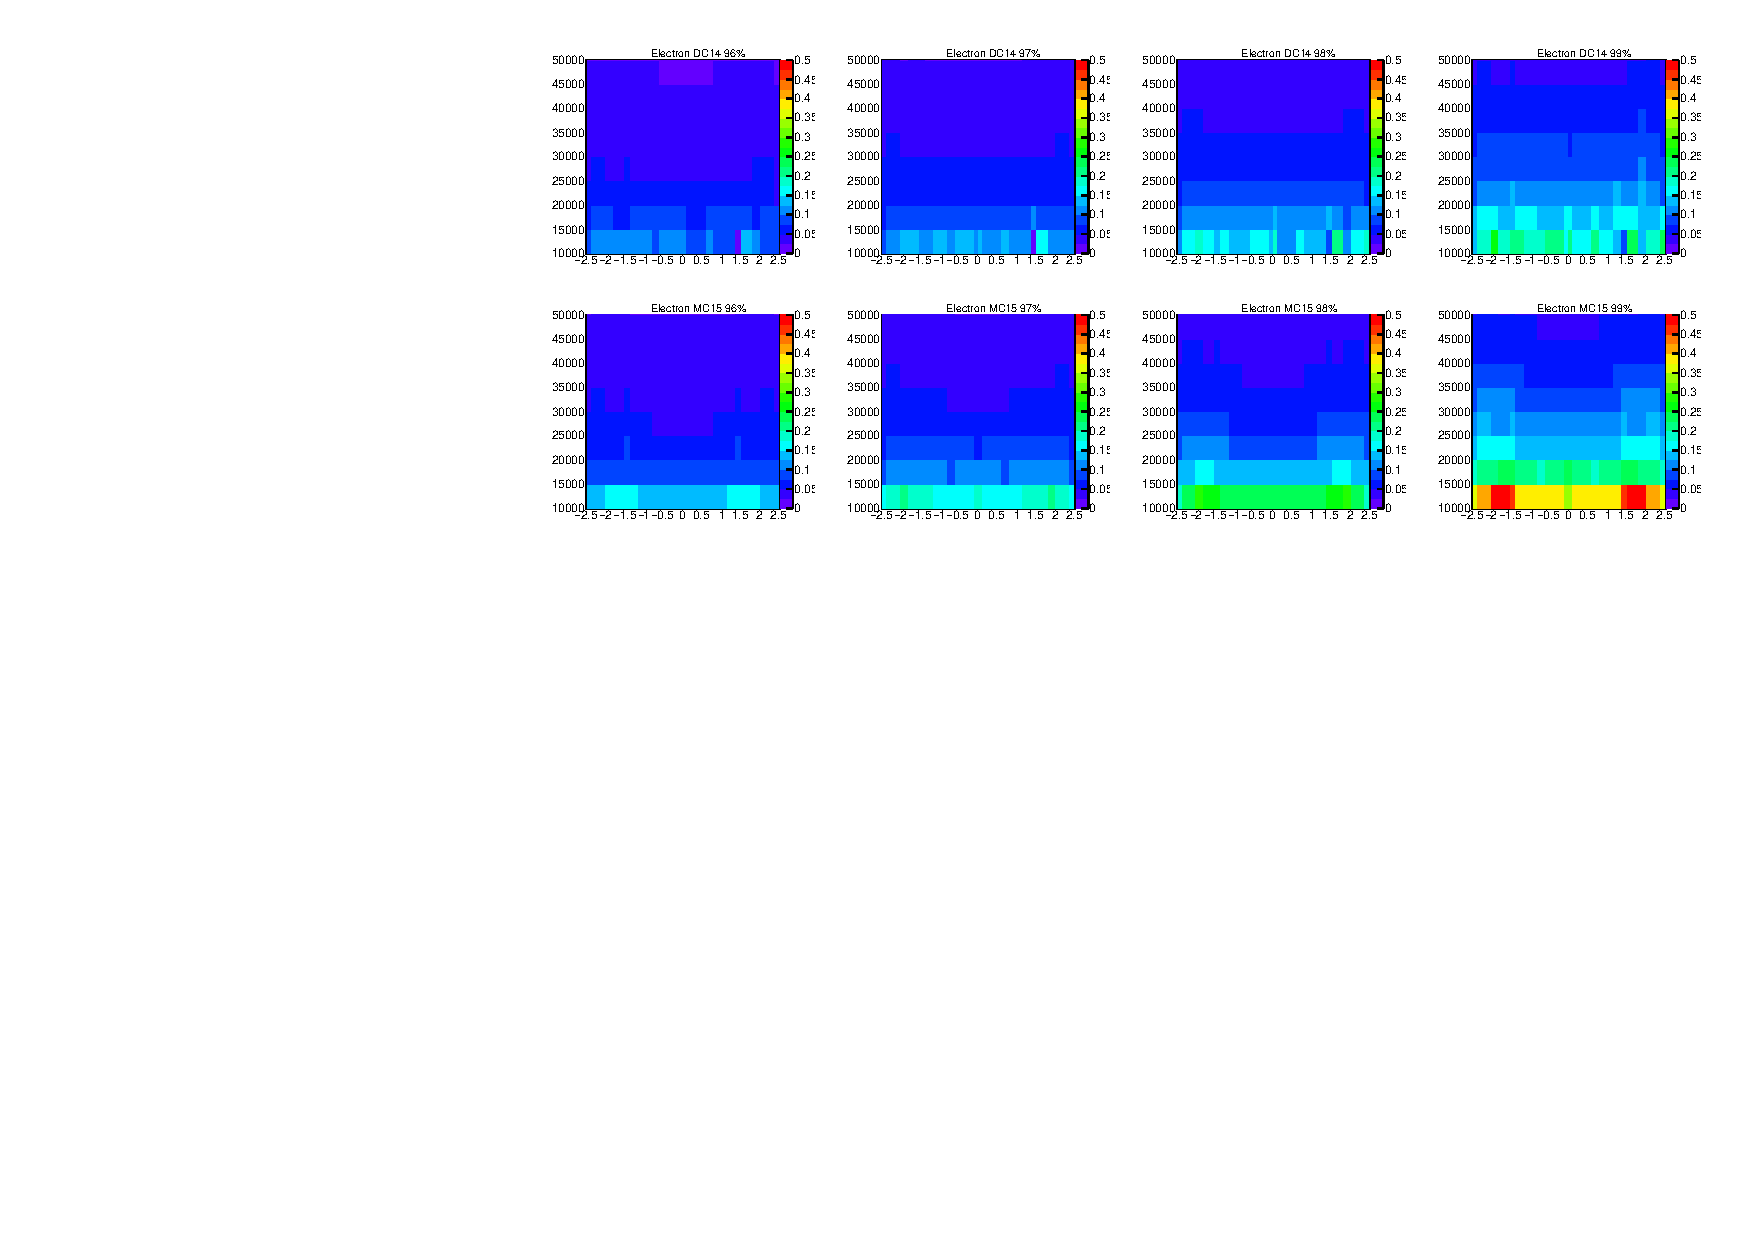
\includegraphics[width=\textwidth]{FIGURES/ISOLATION/Electron_ptvarcone20.pdf}
\end{center}
\vspace{-0.2cm}
\caption{Thresholds on the ptvarcone20/\pt used for the electron isolation working points in the DC14 pre-pre-recommendations (top) and in the MC15 pre-recommendations(bottom). These thresholds are shown as a function of the electron \pt and \eta for isolation efficiency of 96-99\%.}
\label{fig:isoThresholdsEleTrk}
\end{figure}


\begin{figure}[phtb!]
\begin{center}
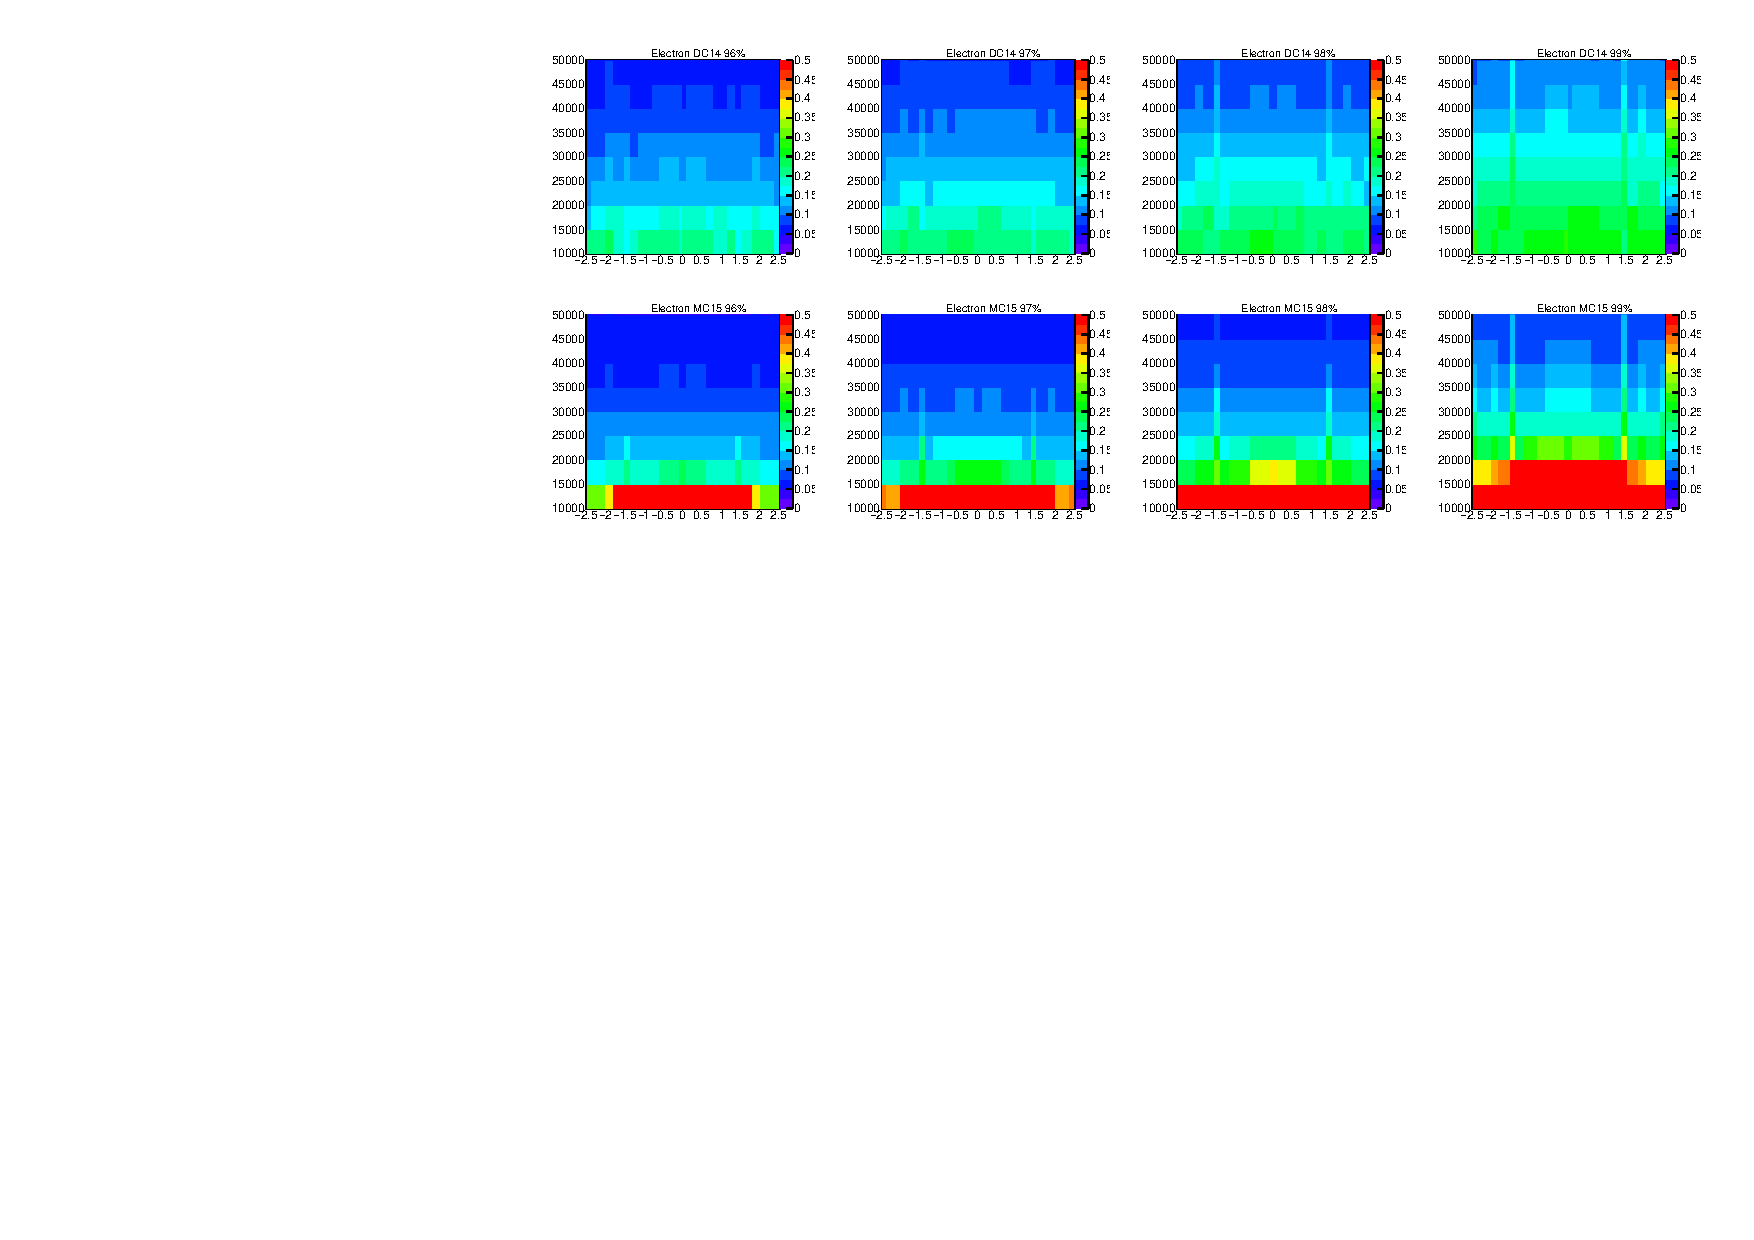
\includegraphics[width=\textwidth]{FIGURES/ISOLATION/Electron_topoetcone20.pdf}
\end{center}
\vspace{-0.2cm}
\caption{Thresholds on the topoetcone20/\pt used for the electron isolation working points in the DC14 pre-pre-recommendations (top) and in the MC15 pre-recommendations(bottom). These thresholds are shown as a function of the electron \pt and \eta for isolation efficiency of 96-99\%.}
\label{fig:isoThresholdsEleCalo}
\end{figure}



\begin{figure}[phtb!]
\begin{center}
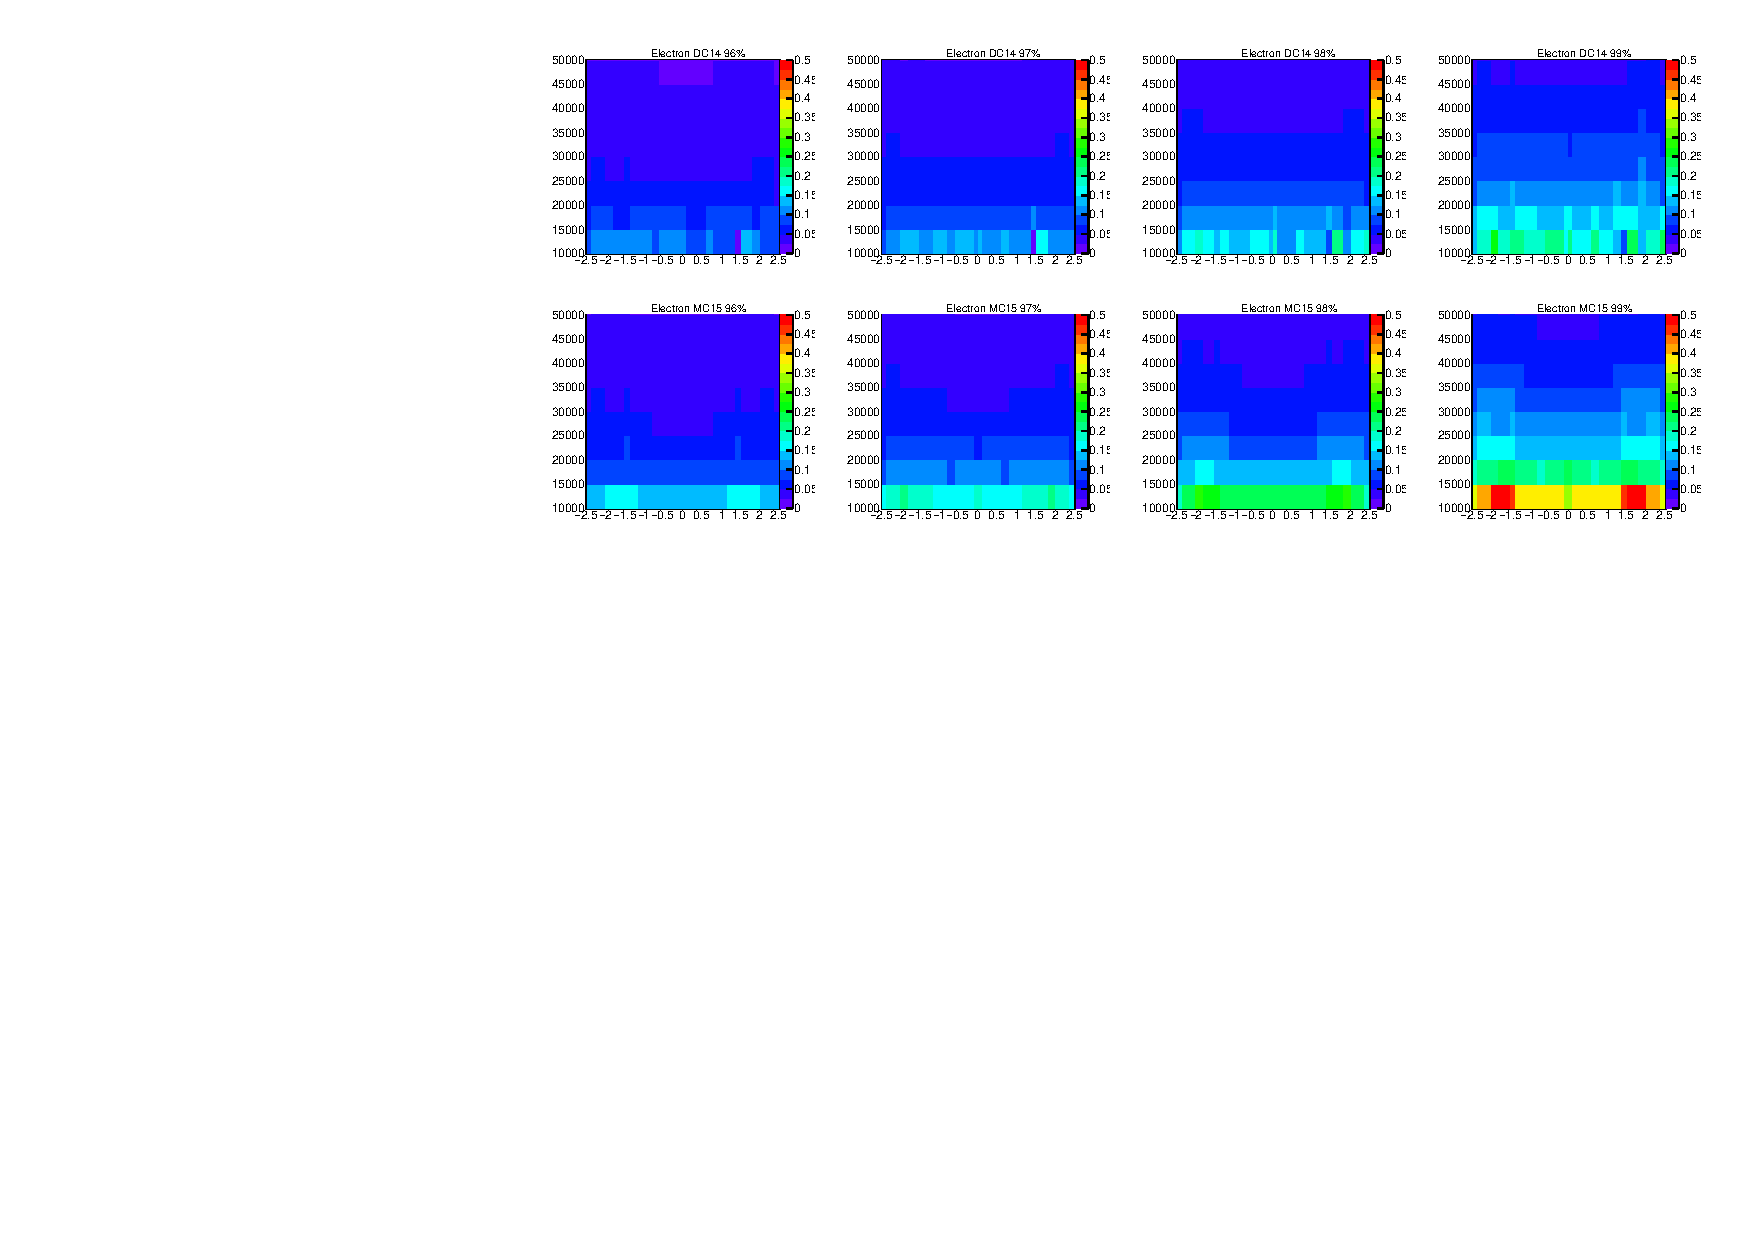
\includegraphics[width=\textwidth]{FIGURES/ISOLATION/Electron_ptvarcone20.pdf}
\end{center}
\vspace{-0.2cm}
\caption{Thresholds on the ptvarcone30/\pt used for the muon isolation working points in the DC14 pre-pre-recommendations (top) and in the MC15 pre-recommendations(bottom). These thresholds are shown as a function of the muon \pt and \eta for isolation efficiency of 96-99\%. }
\label{fig:isoThresholdsMuTrk}
\end{figure}


\begin{figure}[phtb!]
\begin{center}
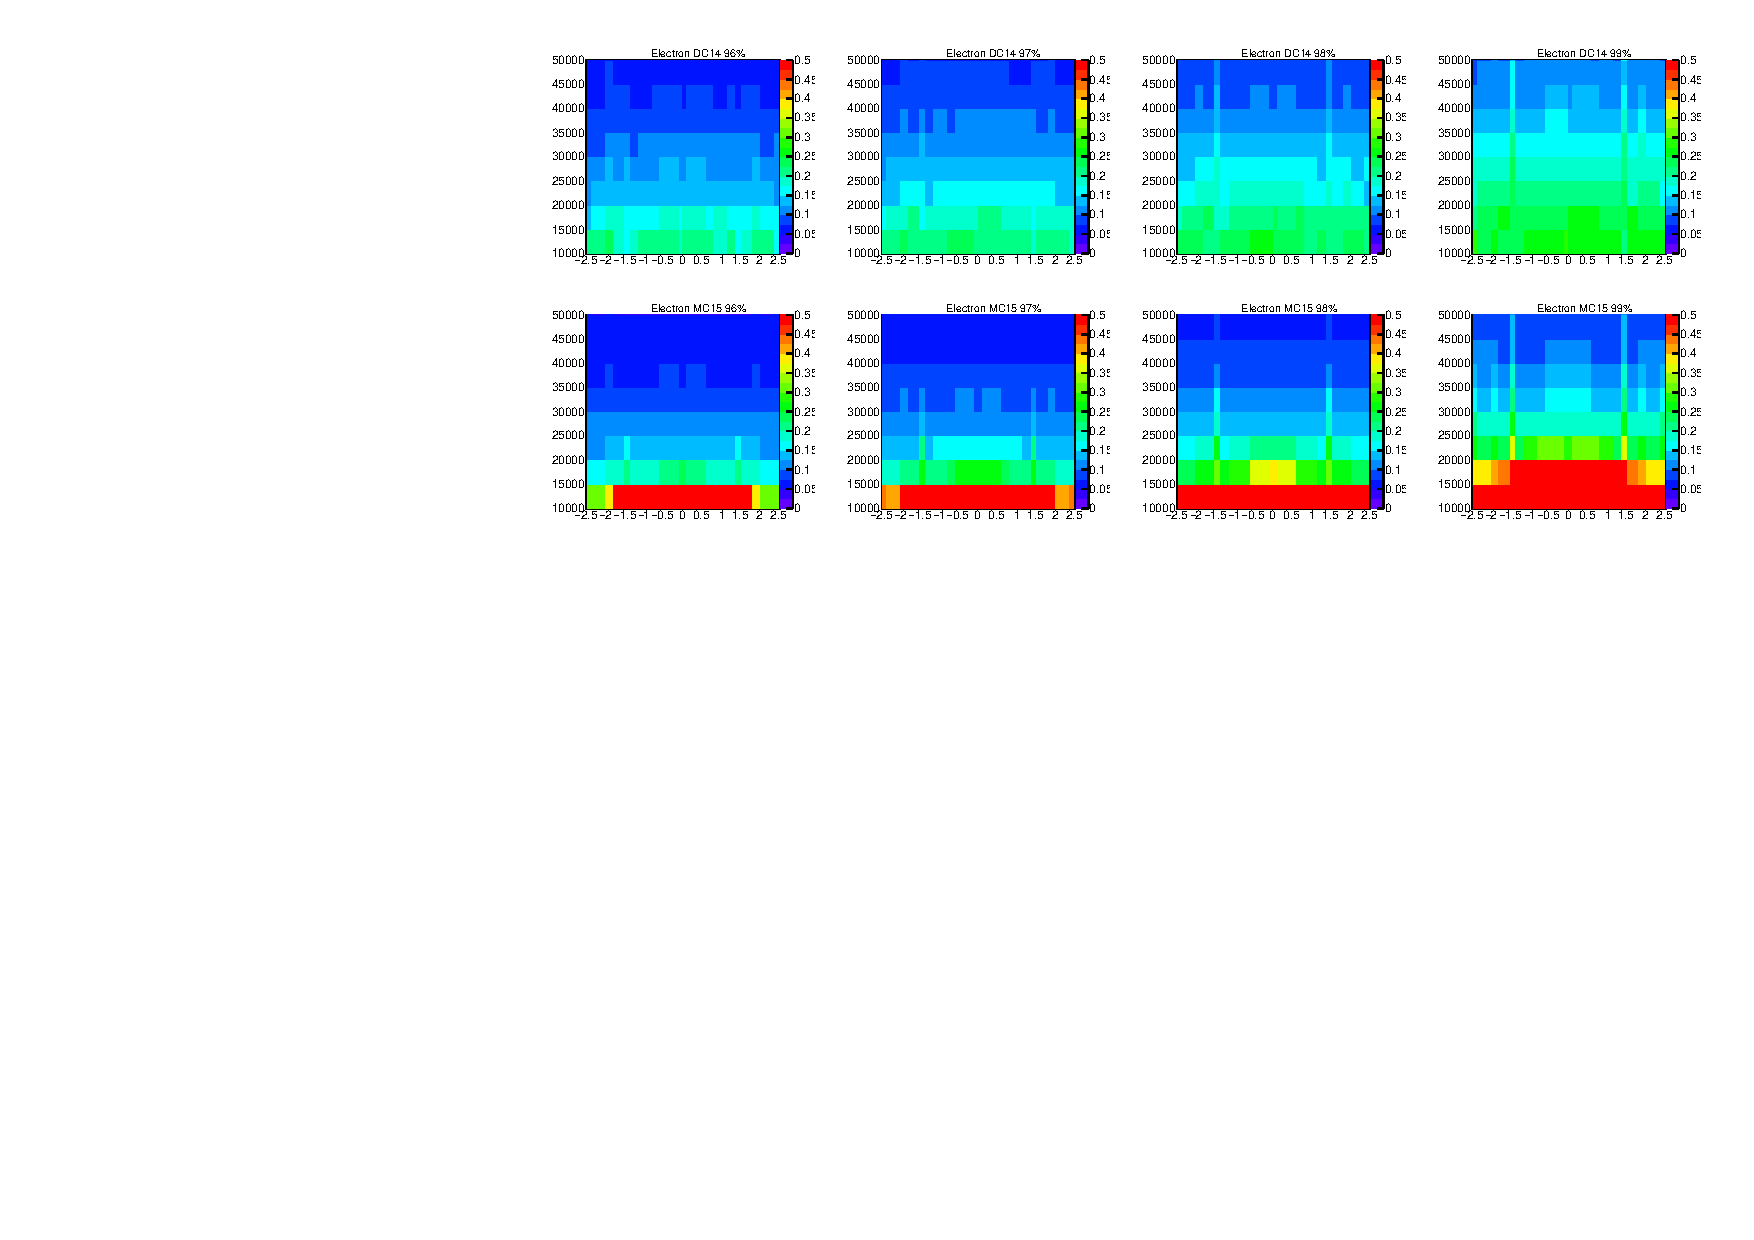
\includegraphics[width=\textwidth]{FIGURES/ISOLATION/Electron_topoetcone20.pdf}
\end{center}
\vspace{-0.2cm}
\caption{Thresholds on the topoetcone20/\pt used for the muon isolation working points in the DC14 pre-pre-recommendations (top) and in the MC15 pre-recommendations(bottom). These thresholds are shown as a function of the muon \pt and \eta for isolation efficiency of 96-99\%. }
\label{fig:isoThresholdsMuCalo}
\end{figure}
